% no answer key
% \documentclass[letterpaper]{exam}

% answer key
\documentclass[letterpaper, landscape]{exam}
\usepackage{2in1, lscape} 
\printanswers

\usepackage{units} 
\usepackage{xfrac} 
\usepackage[fleqn]{amsmath}
\usepackage{float}
\usepackage{mdwlist}
\usepackage{booktabs}
\usepackage{cancel}
\usepackage{polynom}
\usepackage{caption}
\usepackage{fullpage}
\usepackage{comment}
\usepackage{enumerate}
\usepackage{graphicx}

\usepackage{mathtools} 

\newcommand{\dg}{\ensuremath{^\circ}} 
\newcommand{\sgn}{\operatorname{sgn}}

\everymath{\displaystyle}
\title{Calculus I \\ Homework Six \\ Section 2.6}
\author{}
\date{\today}

\begin{document}

  \maketitle

  \section{Homework}
    \begin{itemize*}
      \item read Section 2.6
      \item exercises: 3-4, 15-33, 39-43, 48
    \end{itemize*}

  \ifprintanswers

  \section{Solutions}

    \begin{description}

      \item[3] 
        \begin{enumerate}[(a)]
          \item $\lim_{x \to 2} f(x) = \infty$
          \item $\lim_{x \to 1^-} f(x) = \infty$
          \item $\lim_{x \to 1^+} f(x) = -\infty$
          \item $\lim_{x \to \infty} f(x) = 1$
          \item $\lim_{x \to -\infty} f(x) = 2$

          \item The vertical asymptotes are at $x = -1$ and $x = 2$
            The horizontal asymptotes are at $y = 1$ and $y = 2$.

        \end{enumerate}

      \item[4] 
        \begin{enumerate}[(a)]
          \item $\lim_{x \to \infty} g(x) = 2$

          \item $\lim_{x \to -\infty} g(x) = -2$

          \item $\lim_{x \to 3} g(x) = \infty$

          \item $\lim_{x \to 0} g(x) = -\infty$

          \item $\lim_{x \to -2^+} g(x) = -\infty$

          \item The vertical asymptotes are at $x = -2$, $x = 0$ and $x = 3$.

            The horizontal asymptotes are at $y = -2$ and $y = 2$.

        \end{enumerate}

      \item[15] 
        $\lim_{x \to \infty} \frac{1}{2x + 3} = \boxed{ 0 }$

      \item[16] 
        $\lim_{x \to \infty} \frac{3x + 5}{x - 4} = \boxed{ 3 }$

      \item[17] 
        $\lim_{x \to -\infty} \frac{1 - x - x^2}{2x^2 - 7} = \boxed{ - \frac{1}{2} }$

      \item[18] 
        $\lim_{y \to \infty} \frac{2 - 3y^2}{5y^2 + 4y} = \boxed{ - \frac{3}{5} }$

      \item[19] 
        $\lim_{x \to \infty} \frac{x^3 + 5x}{2x^3 - x^2 + 4} = \boxed{ \frac{1}{2} }$

      \item[20] 
        $\lim_{t \to -\infty} \frac{t^2 + 2}{t^3 + t^2 - 1} = \boxed{ -1 }$

      \item[21] 
        $\lim_{u \to \infty} \frac{4u^4 + 5}{\left(u^2 - 2 \right) \left(2u^2 - 1 \right)} 
          = \boxed{ 2 }$

      \item[22] 
        $\lim_{x \to \infty} \frac{x + 2}{\sqrt{9x^2 + 1}} = \boxed{ \frac{1}{3} }$

      \item[23] 
        $\lim_{x \to \infty} \frac{\sqrt{9x^6 - x}}{x^3 + 1} = \boxed{ 3 }$

      \item[24] 
        $\lim_{x \to -\infty} \frac{\sqrt{9x^6 - x}}{x^3 + 1} = \boxed{ -3 }$

      \item[25] 
        $\lim_{x \to \infty} \left( \sqrt{9x^2 + x} - 3x \right) 
          = \boxed{ \frac{1}{6} }$

      \item[26] 
        $\lim_{x \to -\infty} \left( x + \sqrt{x^2 + 2x} \right) = \boxed{ -1 }$

      \item[27] 
        $\lim_{x \to \infty} \left( \sqrt{x^2 + ax} - \sqrt{x^2 + bx} \right) 
          = \boxed{ \frac{1}{2} (b - a) }$

      \item[28] 
        $\lim_{x \to -\infty} \cos x$ does not exist.

      \item[29] 
        $\lim_{x \to \infty} \frac{x + x^3 + x^5}{1 - x^2 + x^4} = \boxed{ \infty }$

      \item[30] 
        $\lim_{x \to \infty} \sqrt{x^2 + 1} = \boxed{ \infty }$

      \item[31] 
        $\lim_{x \to -\infty} \left( x^4 + x^5 \right) = \boxed{ -\infty }$

      \item[32] 
        $\lim_{x \to \infty} \frac{x^3 - 2x + 3}{5 - 2x^2} = \boxed{ -\infty }$

      \item[33] 
        $\lim_{x \to \infty} \frac{1 - e^x}{1 + 2e^x} = \boxed{ - \frac{1}{2} }$

      \item[39]
        \begin{tabular}[H]{ll}
          \toprule
          Horizontal Asymptotes & $y = 2$ \\
          Vertical Asymptotes   & $x = 2$ \\
          \bottomrule
        \end{tabular}

        \begin{figure}[H]
          \centering
          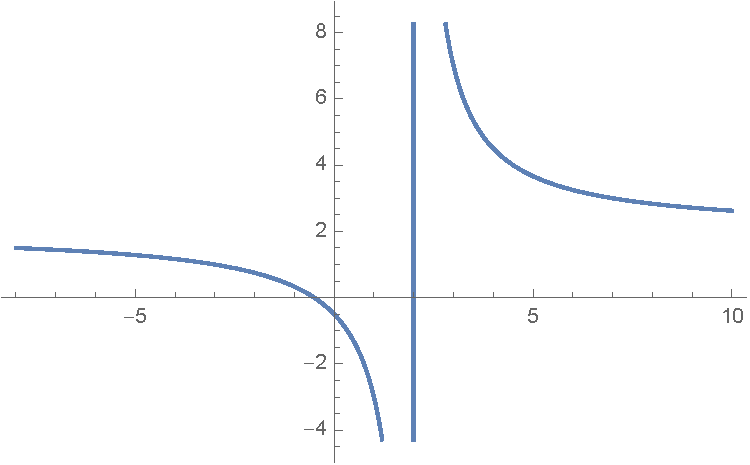
\includegraphics[scale = 0.5]{ex39.pdf}
          \caption{Exercise 39}
          \label{fig:ex39}
        \end{figure}

      \item[40]
        \begin{tabular}[H]{ll}
          \toprule
          Horizontal Asymptotes & $y = \frac{1}{2}$ \\
          Vertical Asymptotes   & $x = - \frac{1}{2}$ and $x = 2$ \\
          \bottomrule
        \end{tabular}

        \begin{figure}[H]
          \centering
          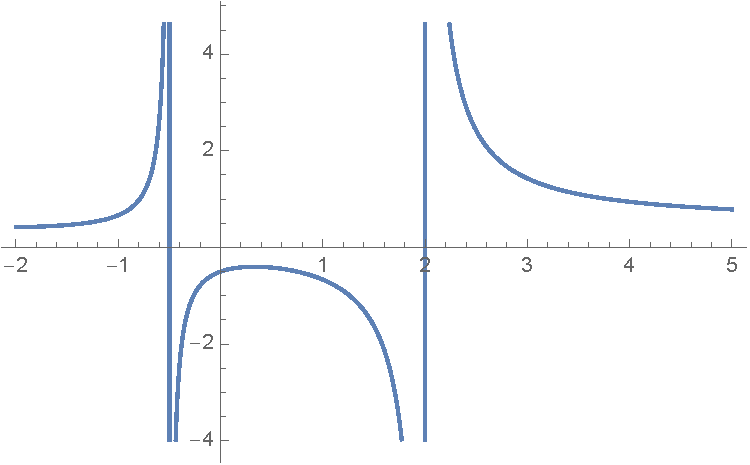
\includegraphics[scale = 0.5]{ex40.pdf}
          \caption{Exercise 40}
          \label{fig:ex40}
        \end{figure}

      \item[41]
        \begin{tabular}[H]{ll}
          \toprule
          Horizontal Asymptotes & $y = 2$ \\
          Vertical Asymptotes   & $x = -2$ and $x = 1$ \\
          \bottomrule
        \end{tabular}

        \begin{figure}[H]
          \centering
          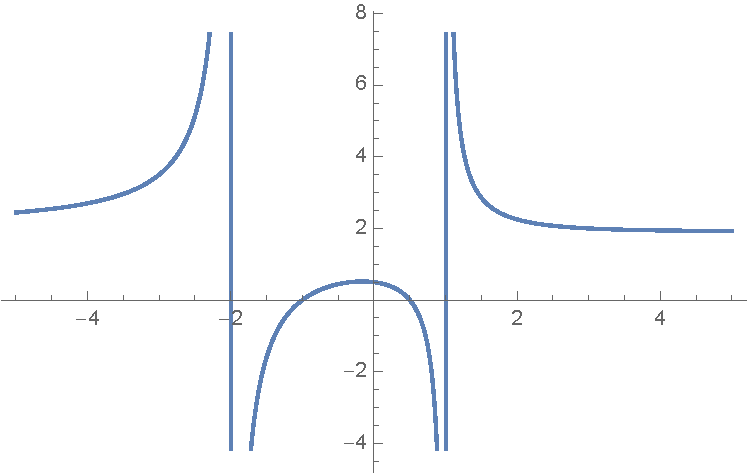
\includegraphics[scale = 0.5]{ex41.pdf}
          \caption{Exercise 41}
          \label{fig:ex41}
        \end{figure}

      \item[42]
        \begin{tabular}[H]{ll}
          \toprule
          Horizontal Asymptotes & $y = 1$ \\
          Vertical Asymptotes   & $x = -1$, $x = 0$ and $x = 1$ \\
          \bottomrule
        \end{tabular}

        \begin{figure}[H]
          \centering
          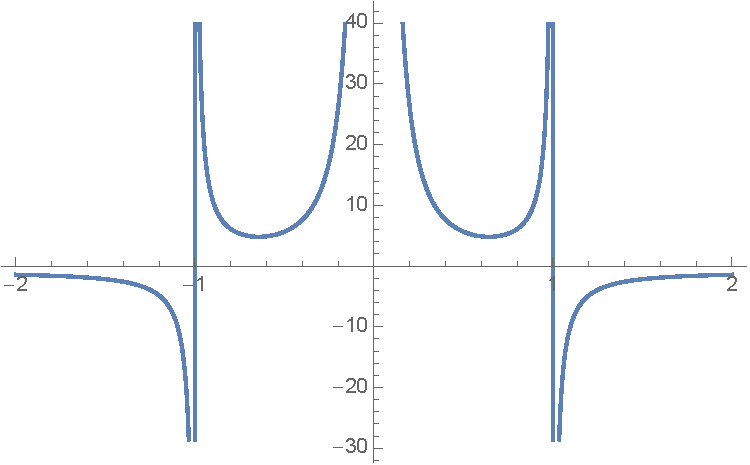
\includegraphics[scale = 0.5]{ex42.pdf}
          \caption{Exercise 42}
          \label{fig:ex42}
        \end{figure}

      \item[43]
        \begin{tabular}[H]{ll}
          \toprule
          Horizontal Asymptotes & none \\
          Vertical Asymptotes   & $x = 5$ \\
          \bottomrule
        \end{tabular}

        $f(x)$ is undefined at $x = 1$ but there isn't an asymptote there because the
        $(x - 1)$ terms in the numerator and denominator cancel and 
        $\lim_{x \to 1} f(x) = -\frac{1}{2}$.

        \begin{figure}[H]
          \centering
          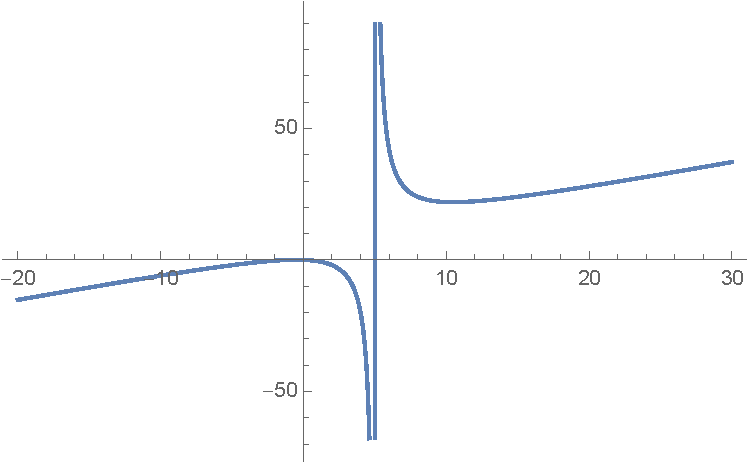
\includegraphics[scale = 0.5]{ex43.pdf}
          \caption{Exercise 43}
          \label{fig:ex43}
        \end{figure}

      \item[48] For there to be vertical asymptotes and $x = 1$ and $x = 3$, the
        denominator should contain the terms $(x - 1)$ and $(x - 3)$.

        For there to be a horizontal asymptote at $x = 1$, the numerator and denominator
        must be the same degree and have the same leading coefficient.

        The simplest function that works is:
        \[
          \boxed{ f(x) = \frac{x^2}{x^2 - 4x + 3} }
        \]
    \end{description}

  \else
    \vspace{10 cm}
    \begin{quote}
      \begin{em}
        Wanton killing of innocent civilians is terrorism, not a ``war against
        terrorism.'' 
      \end{em}
    \end{quote}
    \hspace{1 cm} --Noam Chomsky
  \fi

\end{document}

